\documentclass[tikz,border=5pt]{standalone}
\usepackage{fontspec}
\setmainfont{Times New Roman}
\usepackage{unicode-math}
\setmathfont{Cambria Math}
\usetikzlibrary{shapes.geometric,positioning,fit,backgrounds,arrows.meta,calc}

\begin{document}
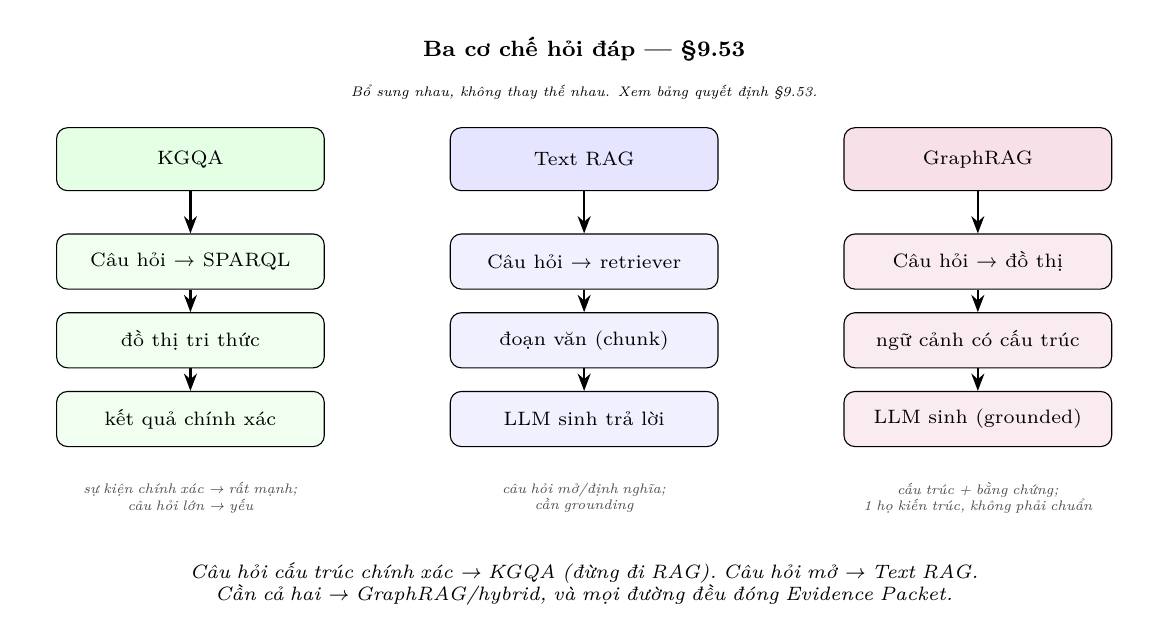
\begin{tikzpicture}[
  box/.style={rectangle, draw, rounded corners, align=center, font=\scriptsize, inner sep=3pt},
  arrow/.style={-{Stealth[length=2.2mm]}, thick},
  label/.style={font=\tiny\itshape, text=gray!60!black},
]

\node[font=\footnotesize\bfseries] at (0, 3.6) {Ba cơ chế hỏi đáp — §9.53};
\node[font=\tiny\itshape] at (0, 3.05) {Bổ sung nhau, không thay thế nhau. Xem bảng quyết định §9.53.};

% === KGQA ===
\node[box, fill=green!10, minimum width=3.4cm, minimum height=0.8cm] (k1) at (-5.0, 2.2) {KGQA};
\node[box, fill=green!6, minimum width=3.4cm, minimum height=0.7cm] (k2) at (-5.0, 0.9) {Câu hỏi → SPARQL};
\node[box, fill=green!6, minimum width=3.4cm, minimum height=0.7cm] (k3) at (-5.0, -0.1) {đồ thị tri thức};
\node[box, fill=green!6, minimum width=3.4cm, minimum height=0.7cm] (k4) at (-5.0, -1.1) {kết quả chính xác};
\draw[arrow] (k1) -- (k2);
\draw[arrow] (k2) -- (k3);
\draw[arrow] (k3) -- (k4);
\node[label, align=center, text width=3.9cm] at (-5.0, -2.1) {sự kiện chính xác → rất mạnh;\\câu hỏi lớn → yếu};

% === Text RAG ===
\node[box, fill=blue!10, minimum width=3.4cm, minimum height=0.8cm] (r1) at (0, 2.2) {Text RAG};
\node[box, fill=blue!6, minimum width=3.4cm, minimum height=0.7cm] (r2) at (0, 0.9) {Câu hỏi → retriever};
\node[box, fill=blue!6, minimum width=3.4cm, minimum height=0.7cm] (r3) at (0, -0.1) {đoạn văn (chunk)};
\node[box, fill=blue!6, minimum width=3.4cm, minimum height=0.7cm] (r4) at (0, -1.1) {LLM sinh trả lời};
\draw[arrow] (r1) -- (r2);
\draw[arrow] (r2) -- (r3);
\draw[arrow] (r3) -- (r4);
\node[label, align=center, text width=3.9cm] at (0, -2.1) {câu hỏi mở/định nghĩa;\\cần grounding};

% === GraphRAG ===
\node[box, fill=purple!12, minimum width=3.4cm, minimum height=0.8cm] (g1) at (5.0, 2.2) {GraphRAG};
\node[box, fill=purple!8, minimum width=3.4cm, minimum height=0.7cm] (g2) at (5.0, 0.9) {Câu hỏi → đồ thị};
\node[box, fill=purple!8, minimum width=3.4cm, minimum height=0.7cm] (g3) at (5.0, -0.1) {ngữ cảnh có cấu trúc};
\node[box, fill=purple!8, minimum width=3.4cm, minimum height=0.7cm] (g4) at (5.0, -1.1) {LLM sinh (grounded)};
\draw[arrow] (g1) -- (g2);
\draw[arrow] (g2) -- (g3);
\draw[arrow] (g3) -- (g4);
\node[label, align=center, text width=3.9cm] at (5.0, -2.1) {cấu trúc + bằng chứng;\\1 họ kiến trúc, không phải chuẩn};

\node[font=\scriptsize\itshape, align=center, text width=12.5cm] at (0, -3.2)
  {Câu hỏi cấu trúc chính xác → KGQA (đừng đi RAG). Câu hỏi mở → Text RAG.\\Cần cả hai → GraphRAG/hybrid, và mọi đường đều đóng Evidence Packet.};

\end{tikzpicture}
\end{document}